%%%%%%%%%%%%%%%%%%%%%%%%%%%%%%%%%%%%%%%%%%%%%%%%%%%%%%%%%%%%%%%%%%%%%%
%
% MARENTIS LABS MASTER POLICY TEMPLATE (v1.7)
%
% NOTES:
% 1. This document MUST be compiled with LuaLaTeX or XeLaTeX
%    to correctly load the 'Inter' font.
% 2. All logo image files must be in the same directory.
% 3. This template uses a custom label for page counting.
%    You MUST run LaTeX twice to ensure page count is correct.
%
%%%%%%%%%%%%%%%%%%%%%%%%%%%%%%%%%%%%%%%%%%%%%%%%%%%%%%%%%%%%%%%%%%%%%%

\documentclass[11pt, a4paper]{article}

% --- PACKAGES ---
\usepackage{geometry}           % For page margins
\usepackage{graphicx}           % For images
\usepackage[HTML]{xcolor}       % For brand colours
\usepackage{fontspec}           % For custom fonts (Inter)
\usepackage{fancyhdr}           % For headers and footers
\usepackage{titlesec}           % For custom section titles
\usepackage{booktabs}           % For professional tables
\usepackage{hyperref}           % For clickable links and ToC
\usepackage{background}         % For the watermark/background logo
% \usepackage{lastpage}         % REMOVED - Replaced with manual label
\usepackage{enumitem}           % For custom lists
\usepackage[toc,page]{appendix} % For annexures
\usepackage{tabularx}			% For flexible-width tables
\usepackage{array}              % [FIX] Added for >{\...} column formatting
\usepackage{float}              % [FIX] Added to force tables [H]ere
\usepackage{parskip}            % Use paragraph spacing, not indentation
\usepackage{pgfplots}           % For data visualization charts
\pgfplotsset{compat=1.18}       % Ensure modern compatibility for pgfplots

% --- BRANDING & FONT SETUP ---
%
% Define Marentis Labs brand colours
\definecolor{ml-charcoal}{HTML}{212529}
\definecolor{ml-slate-grey}{HTML}{495057}
\definecolor{ml-gold}{HTML}{a98c5a}
\definecolor{ml-slate-blue}{HTML}{4a6572}
\definecolor{ml-light-bg}{HTML}{f8f9fa}

% Set main font to Inter
\setmainfont{Inter}
\setsansfont{Inter}

% Set hyperlink colours
\hypersetup{
    colorlinks=true,
    linkcolor=ml-slate-blue,
    urlcolor=ml-slate-blue,
    citecolor=ml-slate-grey,
}

% --- Custom Page Style for Final Page (v1.7) ---
\fancypagestyle{companyinfo}{
    \fancyhf{} % Clear all fields
    \fancyfoot[L]{
\includegraphics[height=1.2cm]{Marentis Mini Logo.png}} % Add logo
    \fancyfoot[R]{} % Ensure page number field is blank
    \renewcommand{\headrulewidth}{0pt} % No header rule
    \renewcommand{\footrulewidth}{0.4pt} % Keep footer rule
}

% --- PAGE LAYOUT & GEOMETRY ---
% Clean, modern margins
\geometry{
    a4paper,
    margin=2.5cm,
    headheight=2.5cm % Generous headheight for the logo
}

% --- SECTION TITLE STYLING ---
%
% Direct, clean, no "empty flair"
\titleformat{\section}
    {\Large\bfseries\color{ml-charcoal}} % Format
    {\thesection.}                      % Label
    {1em}                               % Sep
    {}                                  % Before-code
\titleformat{\subsection}
    {\large\bfseries\color{ml-slate-grey}}
    {\thesubsection.}
    {1em}
    {}

% Spacing for titles
\titlespacing*{\section}{0pt}{3.5ex plus 1ex minus .2ex}{2.3ex plus .2ex}
\titlespacing*{\subsection}{0pt}{3.25ex plus 1ex minus .2ex}{1.5ex plus .2ex}

% --- HEADER & FOOTER SETUP ---
%
\pagestyle{fancy}
\fancyhf{} % Clear all header and footer fields

% Header: NoTag Logo on left, document context on right
%
\fancyhead[L]{\includegraphics[height=1.5cm]{Marentis Labs NoTag Logo.png}}
% --- Generic Header Placeholder ---
\fancyhead[R]{\small\color{ml-slate-grey}Marentis Labs | Carbon Reduction Plan}

% Footer: Mini Logo on left, page number on right
%
\fancyfoot[L]{
\includegraphics[height=1.2cm]{Marentis Mini Logo.png}}
% --- Uses custom \pageref{TrueLastPage} ---
\fancyfoot[R]{\small\color{ml-slate-grey}Page \thepage\ of \pageref{TrueLastPage}}

% Rules
\renewcommand{\headrulewidth}{0.4pt}
\renewcommand{\footrulewidth}{0.4pt}
\renewcommand{\headrule}{\color{ml-slate-blue}\hrule width\headwidth height 0.4pt}
\renewcommand{\footrule}{\color{ml-slate-blue}\hrule width\headwidth height 0.4pt}


% --- DOCUMENT START ---
\begin{document}

% --- COVER PAGE ---
\begin{titlepage}
	\backgroundsetup{contents = {}}    
    \centering
    \vspace*{2cm}
    
    % Use the full logo with tagline
    \includegraphics[width=1.0\textwidth]{Marentis Labs Full Logo.png}
    
    \vfill % Pushes content to vertical center
    
    % Proposal Title
    {\color{ml-charcoal}\Huge\bfseries Corporate Policy Document}
    \\[2ex]
    \vspace{1cm}
    {\color{ml-slate-blue}\Huge\bfseries Carbon Reduction Plan}
    \\[1ex]
    \vspace{0.5cm}
    {\color{ml-slate-grey}\Large\bfseries Commitment to Net Zero by 2050}
    
    \vfill % Pushes content to bottom
    
    % Submission Details
    \large
    \begin{flushleft}
    \parbox{0.5\textwidth}{
        \color{ml-slate-grey}\bfseries Version Number:\\[1ex]
        \color{ml-charcoal}1.0
        \\[4ex]
        \color{ml-slate-grey}\bfseries Effective Date:\\[1ex]
        \color{ml-charcoal}1st January 2026
    }
    \end{flushleft}
    
    \thispagestyle{empty} % No header/footer on cover
\end{titlepage}

% --- TABLE OF CONTENTS ---
\newpage
\pagestyle{empty} % No header/footer on ToC

% --- Special Background for ToC Page ---
%
\backgroundsetup{
    scale=1.6, % "large"
    color=black,
    opacity=0.3, % Still subtle, but more present than the page watermark
    angle=0,
    vshift=0cm,
    contents={
\includegraphics[height=8cm]{Marentis Mini LogoBackground.png}}
}
\BgThispage % Apply this background setup *only* to this page

\renewcommand{\contentsname}{Table of Contents}
{\color{ml-charcoal}\tableofcontents} % Print the ToC over the background
\thispagestyle{empty}

% --- MAIN PROPOSAL CONTENT ---
\newpage
\pagestyle{fancy} % Activate the header/footer
\pagenumbering{arabic} % Start page numbering at 1

% --- WATERMARK SETUP ---
%
% Activate the subtle background logo for all subsequent pages
\backgroundsetup{
    scale=0.9,
    color=black,
    opacity=0.2, % Very subtle
    angle=0,
    vshift=0cm,
    contents={
\includegraphics[width=\paperwidth]{Marentis Mini LogoBackground.png}}
}
\BgThispage % Apply background to current page and all following

% --- SECTION 1 ---
\section{Commitment to Achieving Net Zero}
\label{sec:commitment}

Marentis Labs is committed to achieving Net Zero emissions by 2050 for our UK operations.

% --- SECTION 2 ---
\section{Baseline Emissions Footprint}
\label{sec:baseline}

Baseline emissions are a record of the greenhouse gases that have been produced in the past and were produced prior to the introduction of any strategies to reduce emissions. Baseline emissions are the reference point against which emissions reduction can be measured.

\textbf{Baseline Year: 2025 (First year of incorporation)}

\textbf{Additional details relating to the Baseline emissions calculations:}

Marentis Labs was incorporated in 2025. This first reporting period serves as our baseline. Calculations follow the GHG Reporting Protocol Corporate Standard using the Operational Control approach. Our footprint is characteristic of a lean, asset-light professional services firm.

To allow for institutional scaling, we have calibrated our baseline using an \textbf{Intensity Metric} of emissions per Full-Time Equivalent (FTE) employee. This ensures that our reduction progress is measured against operational efficiency as the firm grows.

\begin{table}[H]
    \centering
    \renewcommand{\arraystretch}{1.5} % Adjust row height
    \begin{tabularx}{\textwidth}{@{} X r @{}}
        \toprule
        \textbf{Emissions} & \textbf{Total (tCO2e)} \\
        \midrule
        \textbf{Scope 1} (Natural Gas) & 1.85 \\
        \textbf{Scope 2} (Purchased Electricity) & 2.10 \\
        \textbf{Scope 3} (Included Sources) & 22.65 \\
        ~~~~* Category 4: Upstream T\&D & 0.25 \\
        ~~~~* Category 5: Waste & 0.20 \\
        ~~~~* Category 6: Business Travel & 15.40 \\
        ~~~~* Category 7: Commuting & 6.80 \\
        ~~~~* Category 9: Downstream T\&D & 0.00 \\
        \midrule
        \textbf{Total Emissions} & \textbf{26.60} \\
        \textbf{Intensity Metric: tCO2e per FTE} & \textbf{2.66} \\
        \bottomrule
    \end{tabularx}
\end{table}

% --- SECTION 3 ---
\section{Current Emissions Reporting}
\label{sec:current_reporting}

\textbf{Reporting Year: 2025}

As 2025 is our first year of operation and our baseline year, the current emissions reporting is identical to the baseline emissions footprint provided in Section \ref{sec:baseline}.

\begin{table}[H]
    \centering
    \renewcommand{\arraystretch}{1.5}
    \begin{tabularx}{\textwidth}{@{} X r @{}}
        \toprule
        \textbf{Emissions} & \textbf{Total (tCO2e)} \\
        \midrule
        \textbf{Scope 1} & 1.85 \\
        \textbf{Scope 2} & 2.10 \\
        \textbf{Scope 3} (Included Sources) & 22.65 \\
        \midrule
        \textbf{Total Emissions} & \textbf{26.60} \\
        \bottomrule
    \end{tabularx}
\end{table}

\begin{figure}[H]
    \centering
    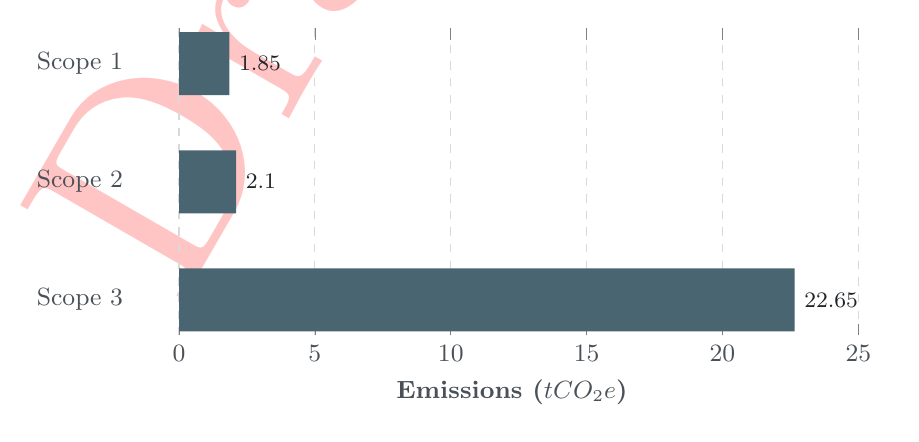
\begin{tikzpicture}
        \begin{axis}[
            xbar,
            y=-1.5cm,
            bar width=0.8cm,
            enlarge y limits=0.3,
            enlargelimits=0.15,
            xlabel={Emissions ($tCO_2e$)},
            symbolic y coords={Scope 1, Scope 2, Scope 3},
            ytick=data,
            nodes near coords,
            nodes near coords align={horizontal},
            every node near coord/.append style={font=\footnotesize\bfseries, color=ml-charcoal},
            ytick style={draw=none},
            axis line style={draw=none},
            xmajorgrids=true,
            grid style={dashed, gray!30},
            width=0.9\textwidth,
            height=6cm,
            tick label style={font=\small, color=ml-slate-grey},
            label style={font=\small\bfseries, color=ml-slate-grey},
            ]
            \addplot[fill=ml-slate-blue, draw=none] coordinates {
                (1.85,Scope 1)
                (2.10,Scope 2)
                (22.65,Scope 3)
            };
        \end{axis}
    \end{tikzpicture}
    \vspace{-0.5em}
    \caption{\small \textit{2025 Baseline Emissions Footprint by Scope.}}
\end{figure}

% --- SECTION 4 ---
\section{Emissions Reduction Targets}
\label{sec:reduction_targets}

Marentis Labs recognises that as a high-growth advisory firm, our absolute headcount is projected to increase. To ensure sustainable growth, we have adopted an \textbf{Intensity-Based Reduction Target} alongside our absolute commitment.

We project that our carbon intensity will decrease from \textbf{2.66 tCO2e/FTE} to \textbf{1.33 tCO2e/FTE} by 2030. This represents a \textbf{50\% increase in carbon efficiency} per employee.

By prioritising intensity metrics, we ensure that every new associate or engagement manager joining Marentis Labs adheres to a progressively lower carbon threshold, ultimately reaching Net Zero (Neutralisation) by 2050.

\begin{figure}[H]
    \centering
    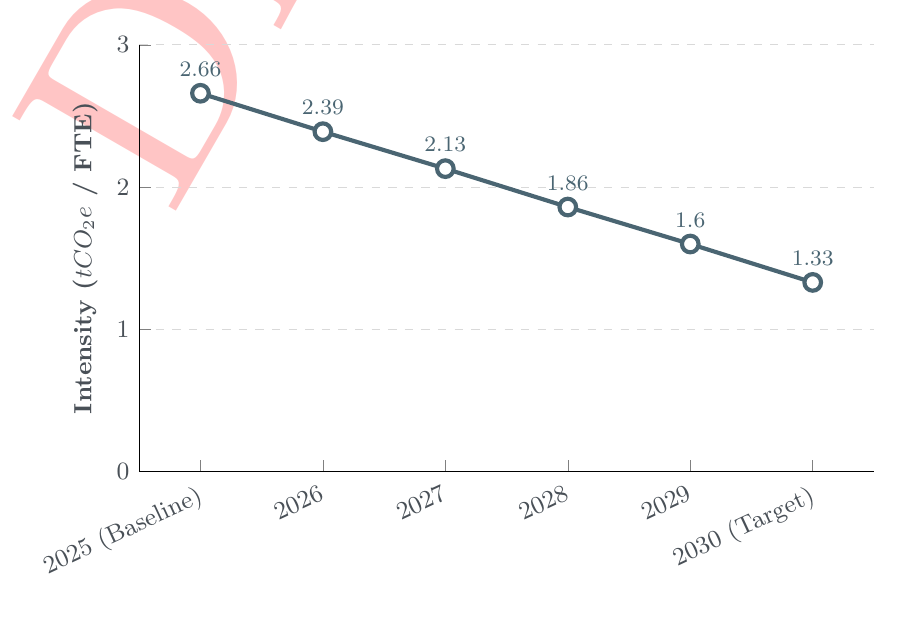
\begin{tikzpicture}
        \begin{axis}[
            width=0.9\textwidth,
            height=7cm,
            symbolic x coords={2025 (Baseline), 2026, 2027, 2028, 2029, 2030 (Target)},
            xtick=data,
            ymin=0, ymax=3.0,
            ylabel={Intensity ($tCO_2e$ / FTE)},
            nodes near coords,
            every node near coord/.append style={font=\footnotesize, yshift=2pt},
            ymajorgrids=true,
            grid style={dashed, gray!30},
            axis x line*=bottom,
            axis y line*=left,
            tick label style={font=\small, color=ml-slate-grey},
            label style={font=\small\bfseries, color=ml-slate-grey},
            xticklabel style={rotate=25, anchor=north east},
            ]
            
            % Pathway projection (Linear for simplicity)
            \addplot[
                color=ml-slate-blue,
                mark=*,
                mark options={fill=white, scale=1.5},
                line width=1.5pt
            ] coordinates {
                (2025 (Baseline), 2.66)
                (2026, 2.39)
                (2027, 2.13)
                (2028, 1.86)
                (2029, 1.60)
                (2030 (Target), 1.33)
            };
        \end{axis}
    \end{tikzpicture}
    \vspace{-0.5em}
    \caption{\small \textit{Projected Intensity Reduction Pathway through 2030.}}
\end{figure}

% --- SECTION 5 ---
\section{Carbon Reduction Projects}
\label{sec:reduction_projects}

\subsection{Completed Carbon Reduction Initiatives}

The following environmental management measures and projects have been implemented during our first year of operation (2025). These measures are in effect when performing the contract.

\begin{itemize}
    \item \textbf{Virtual Presence Policy:} Management has implemented a "Digital-First Discovery" mandate for all initial institutional scoping phases to minimise the requirement for high-carbon business travel.
    \item \textbf{Travel Hierarchy Optimisation:} Strengthening our internal travel policy to mandate "Rail-by-Default" for all travel within a 500-mile radius of our operational hub.
    \item \textbf{Supply Chain Engagement:} We will introduce a sustainable procurement policy, requiring our top five service providers by spend to provide evidence of their own carbon reduction initiatives by 2028.
    \item \textbf{Energy Efficiency:} Use of high-efficiency LED lighting and low-power computing infrastructure across all UK operations.
\end{itemize}

\subsection{Future Carbon Reduction Initiatives}

In the future we hope to implement further measures such as:

\begin{itemize}
    \item \textbf{High-Integrity Carbon Offsetting:} From FY2026, Marentis Labs will implement a policy to offset 100\% of residual Scope 6 (Business Travel) emissions. We will prioritise "Gold Standard" or "Verra" certified credits, focusing on nature-based solutions and community-led decarbonisation projects that offer high fiduciary transparency.
    \item \textbf{Supply Chain Audit:} Requiring all key technology service providers to disclose carbon footprints and align with Net Zero targets by 2030.
    \item \textbf{ISO 14001 Alignment:} Implementing a formal Environmental Management System to systematically monitor and reduce our operational footprint.
\end{itemize}

% --- SECTION 6 ---
\section{Declaration and Sign Off}
\label{sec:declaration}

This Carbon Reduction Plan has been completed in accordance with PPN 006 and associated guidance and reporting standard for Carbon Reduction Plans.

Emissions have been reported and recorded in accordance with the published reporting standard for Carbon Reduction Plans and the GHG Reporting Protocol corporate standard and uses the appropriate Government emission conversion factors for greenhouse gas company reporting.

While Marentis Labs does not currently fall within the statutory scope of Streamlined Energy and Carbon Reporting (SECR), Scope 1 and Scope 2 emissions have been voluntarily calculated in accordance with SECR methodologies to ensure the highest standard of fiduciary transparency. The required subset of Scope 3 emissions has been reported in accordance with the published reporting standard for Carbon Reduction Plans and the Corporate Value Chain (Scope 3) Standard.

This Carbon Reduction Plan has been reviewed and signed off by the Sole Shareholder and Managing Director.

\vspace{1em}
\textbf{Signed on behalf of the Supplier:}

\vspace{0.5em}

\includegraphics[height=1.5cm]{OVSig.png}

\vspace{0.5em}
\textbf{Owen Vallis}

\textbf{Managing Director, Marentis Labs Ltd}

\textbf{Date: 1st January 2026}


% --- ANNEXURES ---
%\begin{appendices}

% \section{[Appendix Title]}
% [Appendix content goes here.]

%\end{appendices}


% --- SET THE 'TRUE LAST PAGE' LABEL ---
% This MUST be placed at the end of the last numbered page
% before the \newpage for the company info.
\label{TrueLastPage} 


% --- FINAL PAGE: COMPANY REGISTRATION ---
%
% Applies the 'companyinfo' pagestyle.
%
\newpage
\thispagestyle{companyinfo} % <--- APPLY THE NEW STYLE (removes page num)

\null % <--- Anchor for the \vfill
\vfill % Pushes the following content to the bottom

\begin{flushleft}
    \scriptsize % <--- FONT SIZE ADJUSTED to 8pt equivalent
    \color{ml-slate-grey} % Set color for all lines
    
    {\bfseries Marentis Labs Ltd} % Bold applied only to this line
    \\[1.5ex]
    Registered in England and Wales
    \\[1ex]
    Company Number: 16600357
    \\[1ex]
    Registered Address: 24 Railfield Gardens, Surrey, RH6 9FY, UK
\end{flushleft}
% The 'companyinfo' footer (logo, no page num) will appear below this.


% --- END OF DOCUMENT ---
\end{document}